% =============================================================================
%  Appendix A — Detailed Corpus Construction Pipeline
% =============================================================================

\section[\appendixname~\thesection]{Detailed Corpus Construction Pipeline}
\label{sec:appendix:corpus_pipeline}

This appendix contains the full procedural detail for the six stages of
corpus construction compressed in Section~\ref{sec:methodology:search} of the
main text. All record counts, tables, and figures reported here are the same
data summarised there; the appendix provides the complete walkthrough for
reproducibility and audit purposes.

\subsection*{A.1 Pre-Validated Corpora (G1--G6)}

In parallel with snowballing, six thematically focused pre-validated corpora
(Groups G1--G6) were assembled through targeted curation of leading
publication venues. Undermind, an AI-assisted academic search tool, was used
to accelerate retrieval of candidate papers from ACL, EMNLP, NeurIPS, ICML,
MLSys, and related venues for each of the six groups. The Undermind queries
are reproduced verbatim in Appendix~B. All inclusion decisions remained with
the human reviewer: Undermind accelerated retrieval of candidates, but
relevance assessment and selection were performed manually.

Because G1--G6 papers were assembled through targeted manual curation, they
bypassed both the year filter and the automated domain-relevance filter
applied to snowballed candidates. Pre-2021 foundational works (e.g.,
Houlsby et al.\ 2019, Hu et al.\ 2022) entered via this route. The year 2021
was adopted as the lower bound for snowballed records because the confluence
of LoRA~\cite{Hu2022} and widespread large-scale transformer deployment marks
the practical onset of the PEFT-at-scale era addressed by this review.

\subsection*{A.2 Citation Snowballing}

Forward and backward citation snowballing was conducted on the G0 seeds
following the procedure of Wohlin et al.~\cite{Wohlin2014}. Backward
snowballing examined the reference lists of each seed; forward snowballing
identified subsequent works citing the seeds. One wave of snowballing was
executed; saturation was assessed qualitatively by inspecting the overlap
between newly retrieved candidates and the pre-validated G1--G6 corpora, with
high overlap suggesting diminishing marginal returns. This was not, however,
formalised as a quantitative stopping criterion (e.g.\ a measured diminishing
marginal inclusion rate); see the discussion of this limitation in
Section~\ref{sec:conclusion:threats}.

Snowballing was executed programmatically via the \textbf{Semantic Scholar
Academic Graph API}~\cite{SemanticScholar2023}, supplemented by the Scopus
(Elsevier) and ACL Anthology engines. The Web of Science Starter API was used
in a post-hoc enrichment role, appending WoS accession numbers and citation
counts to already-retrieved records, not as a source of new candidates. The
search was executed on \textbf{2026-04-21}. In total, 1,150 raw records were
retrieved; after deduplication by DOI and Semantic Scholar paper identifier,
\textbf{972 unique records} entered the title screening stage (178 duplicates
removed).

\subsection*{A.3 Inclusion and Exclusion Criteria}

Eleven of the 123 included records (\textbf{8.9\%}) are arXiv preprints with
no peer-reviewed published venue at the search date; they are included where
they carry a non-trivial external citation count (Semantic Scholar, retrieved
2026-04-21), which serves as a minimal, \emph{external} proxy for
community engagement and peer scrutiny. By this criterion a preprint must have
documented uptake in the wider literature to be retained, independently of
whether it is cited within the review's own corpus. The threshold was set
conservatively low to favour recall, as recent preprints (2025--2026) may not
yet have accumulated citations. The retained preprints span \textbf{2--318}
external citations (median 48); nine have $\geq$10 and four have $\geq$100,
so all eleven comfortably clear any minimal peer-scrutiny proxy. The
implications of this criterion for corpus composition are discussed in
Section~\ref{sec:conclusion:threats}.

\subsection*{A.4 Screening Procedure}

Title screening was applied to all 972 snowballed records in three layers.
\textbf{Layer~1} identified records published before 2021 based on publication
year metadata. \textbf{Layer~2} scored each title against four pre-defined
term sets --- \textit{PEFT/adapters}, \textit{LLM/transformers},
\textit{systems/serving}, and \textit{distributed/P2P/federated} --- using
exact substring matching (term-set version~1.0). Records matching $\geq$2
term sets were flagged for inclusion; records matching exactly one non-LLM
term set were queued for triage; LLM-only matches and zero-match records were
excluded. The author verified all keyword-flagged records during the
subsequent review stages. \textbf{Layer~3} resolved the remaining 130-record
triage queue through manual assessment of title and venue metadata. The author
reviewed all 130 records individually; to support consistency across this
batch, an automated classifier generated preliminary sorting suggestions,
which the author independently verified before finalising each
classification. Records classified as UNCERTAIN (19 of 130) were retained for
closer inspection. The classifier model identifier and per-record decisions
are recorded in the audit log. Table~\ref{tab:screening} shows the screening
outcomes.

\begin{table}[H]
\centering
\caption{Title screening outcomes across the 972 snowballed records, shown by
layer. The bold final counts match the screened records stored in the pipeline
and the audit log.}
\label{tab:screening}
\begin{tabular}{lrr}
\toprule
\textbf{Decision} & \textbf{Layer~2} & \textbf{Layer~3} \\
 & \textbf{(keyword)} & \textbf{(triage)} \\
\midrule
INCLUDE           & 111 & ${+}\,51$ \\
UNCERTAIN         & 130 & $\phantom{+}19$ \\
EXCLUDE           & 731 & ${+}\,60$ \\
\midrule
\textbf{Final INCLUDE}   & \multicolumn{2}{r}{\textbf{162}} \\
\textbf{Final UNCERTAIN} & \multicolumn{2}{r}{\textbf{19}} \\
\textbf{Final EXCLUDE}   & \multicolumn{2}{r}{\textbf{791}} \\
\midrule
\textbf{Total screened}  & \multicolumn{2}{r}{\textbf{972}} \\
\bottomrule
\end{tabular}
\end{table}
\vspace*{-2pt}
\emph{Column totals:} Layer~2 \mbox{111 + 130 + 731 = 972}. Layer~3 resolved
the 130-record triage queue into 51 inclusion, 60 exclusion, and 19 retained
UNCERTAIN; combined with the Layer~2 tallies, $111{+}51{=}162$ INCLUDE and
$731{+}60{=}791$ EXCLUDE. The 19 UNCERTAIN records were re-examined manually after screening: only 3
reached the abstract-level review stage and none was retained in the final
reading list (Section~A.7 in this appendix), so they contributed no records
to the merged corpus or final synthesis. They are therefore not part of the
502-record merged pool, which is drawn solely from the 162 title-screened
INCLUDE records (Table~\ref{tab:screening}).

The automated classifier operated exclusively at the title level, processing
title and venue name only; no abstracts or full-text content were submitted
to the model. All final inclusion and exclusion decisions were made by the
author. The model identifier, term-set version, and per-record decisions are
recorded in the audit log (\texttt{log\_screening\_2026-04-21.json}).

\subsection*{A.5 Enrichment and Tier Classification}

All records passing title screening were merged with the 352-paper
pre-validated corpus (G0--G6) and enriched with full abstracts and keyword
metadata via the Semantic Scholar batch API and OpenAlex. On merge, the 162
title-screened INCLUDE records (162 ${}+{}$ 352 $=$ 514) were
cross-deduplicated against the pre-validated corpus by DOI, arXiv, and
Semantic Scholar identifier: \textbf{12 records} were already present in the
pre-validated corpus and were removed as duplicates, yielding the reported
\textbf{502}-record merged pool (reproducible by re-running
\texttt{app.merge.py}). The 19 UNCERTAIN title-screening records were not part
of this merge (it used only the 162 INCLUDE records) and were excluded at
final curation. A
topical-relevance filter subsequently removed off-topic records (6 excluded)
and deprioritised low-citation arXiv preprints lacking a Tier~1 topic signal
(32 moved to a rescue file). The remaining \textbf{464 records} were
classified into three tiers based on combined title, abstract, and keyword
signal:

\begin{table}[H]
\centering
\caption{Tier classification of the 464-paper enriched corpus.}
\label{tab:tiers}
\begin{tabular}{llrr}
\toprule
\textbf{Tier} & \textbf{Criteria} & \textbf{\textit{N}} & \textbf{\%} \\
\midrule
Tier~1 & PEFT + distributed/P2P + LLM (all three) &  90 & 19.4 \\
Tier~2 & Two of the three themes                  & 141 & 30.4 \\
Tier~3 & Foundational or tangential (one theme)   & 233 & 50.2 \\
\midrule
\textbf{Total} & & \textbf{464} & \\
\bottomrule
\end{tabular}
\end{table}

\begin{figure}[H]
  \centering
  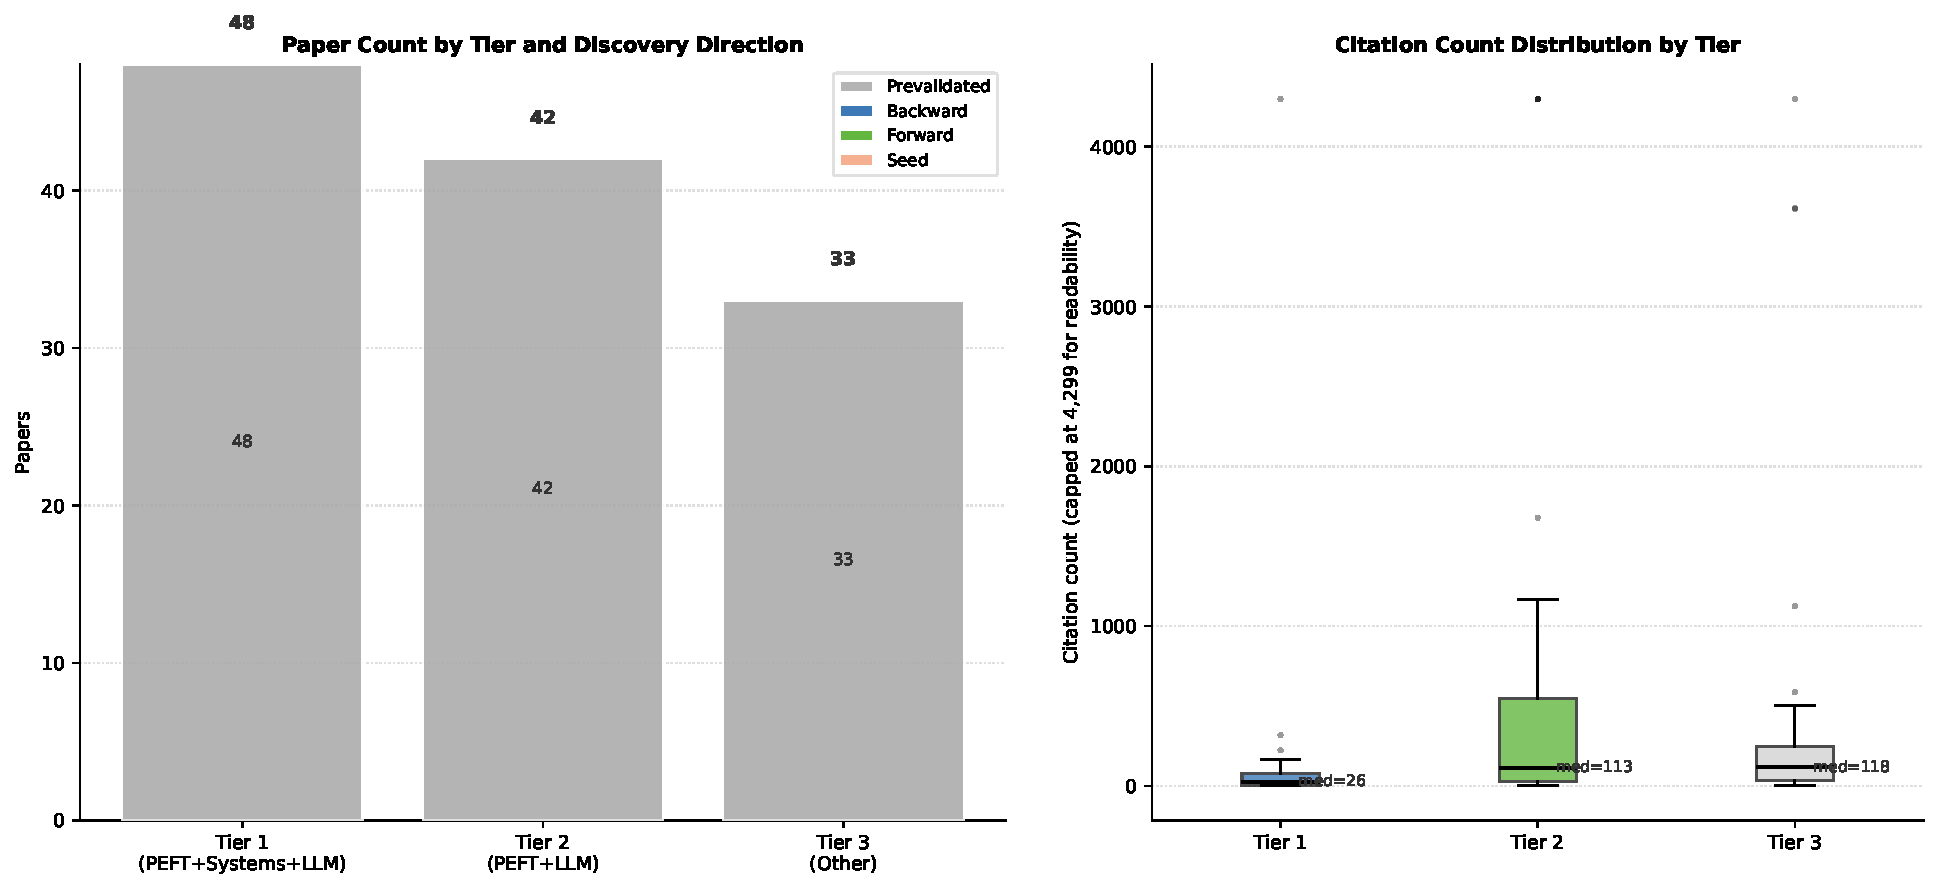
\includegraphics[width=1\linewidth]{figures/fig_slr6_tier_breakdown.pdf}
  \caption{Tier breakdown of the 123-record final list (cf.\ Table~\ref{tab:tiers}
           for the enrichment-stage tiering of the 464-record pool).
           Tier~1 papers (48, 39.0\%) address all three themes;
           Tier~2 (42, 34.1\%) address two;
           Tier~3 (33, 26.8\%) address one theme. The right panel shows the
           citation-count distribution by tier for the 123 records.}
  \label{fig:tiers}
\end{figure}

Tiers (Figure~\ref{fig:tiers}) served as a reading-priority guide following the three-pass method of
Keshav~\cite{Keshav2007}: Tier~1 papers received full reads, Tier~2
selective reads, and Tier~3 abstract-level assessment. Venue quality of the
464-paper corpus: 166 papers (35.8\%) were published in CORE A$^*$ or Scopus
Q1 venues; 189 (40.7\%) in other peer-reviewed conferences or journals; 91
(19.6\%) were arXiv preprints without a published venue; and 18 (3.9\%) had
unknown or missing venue metadata.

Table~\ref{tab:extraction_codebook} documents the column schema of the data
extraction table (`11\_data\_extraction\_2026-05-12.csv`, 224 rows) that feeds
the funnel in Section~\ref{sec:methodology:search}. Coverage reports the number
of the 224 rows carrying a non-null value. Three schema columns
(`method\_name`, `datasets`, `metrics`) are uniformly empty in the archived
export; the quantitative evaluation evidence they were intended to hold is
instead captured narratively in `key\_finding`/`notes\_raw`, and the
corresponding appraisal dimensions are handled in
Section~\ref{sec:methodology:quality}.

\begin{sidewaystable}[p]
\centering
\caption{Data-extraction codebook: column schema, meaning, allowed values, and
coverage of the 224-row extraction table.}
\label{tab:extraction_codebook}
\small
\setlength{\tabcolsep}{4pt}
\begin{tabular}{lp{2.6cm}p{6.4cm}r}
\toprule
\textbf{Column} & \textbf{Meaning} & \textbf{Allowed / typical values} & \textbf{Coverage} \\
\midrule
\texttt{paper\_key} & Internal record key (arXiv ID, DOI, or Scopus hash) & arXiv id / DOI / 40-hex Scopus hash & 223/224 \\
\texttt{arxiv\_id} & arXiv identifier, where applicable & \texttt{YYYY.NNNNN} & 81/224 \\
\texttt{doi} & Digital Object Identifier & DOI string & 185/224 \\
\texttt{title} & Article title & free text & 224/224 \\
\texttt{authors} & Author list & semicolon-separated & 217/224 \\
\texttt{year} & Publication year & 4-digit year & 223/224 \\
\texttt{venue} & Publishing venue & venue name & 221/224 \\
\texttt{citation\_count} & Citations at retrieval (from Crossref/SS) & non-negative integer & 205/224 \\
\texttt{tier} & Reading-priority tier & \texttt{1}/\texttt{2}/\texttt{3} (see Table~\ref{tab:tiers}) & 190/224 \\
\texttt{review\_source} & Whether the record proceeded from full-text or abstract second pass & \texttt{fulltext} / \texttt{abstract-2nd-pass} & 190/224 \\
\texttt{corpus} & Relevance position & \texttt{core} / \texttt{background} & 190/224 \\
\texttt{contribution\_type} & Inferred contribution category & one of 15 categories (per-table text) & 190/224 \\
\texttt{method\_name} & (schema) named method — not populated in archive & free text & 0/224 \\
\texttt{peft\_technique} & PEFT technique used & e.g.\ \texttt{LoRA}, \texttt{bottleneck adapter}, \texttt{prefix}, \texttt{generic-PEFT}, \texttt{none} & 190/224 \\
\texttt{distribution\_mechanism} & How model/adapter state is shared & e.g.\ \texttt{federated}, \texttt{P2P/gossip}, \texttt{centralised server}, \texttt{DHT}, \texttt{none} & 190/224 \\
\texttt{thesis\_sections} & Review sections citing the paper & \texttt{\S n.n} references & 190/224 \\
\texttt{contribution\_codes} & Novel-contribution tag(s) & \texttt{\ccstar A1/S1/R1/R2/T2/M2} combinations & 22/224 \\
\texttt{datasets} & (schema) datasets used — not populated in archive & free text & 0/224 \\
\texttt{metrics} & (schema) evaluation metrics — not populated in archive & free text & 0/224 \\
\texttt{key\_finding} & One-line primary outcome / contribution summary & free text (max ~1--2 lines) & 190/224 \\
\texttt{notes\_raw} & Full-text reading notes (methods, results, \texttt{\S} and \texttt{\ccstar} tags) & free text & 190/224 \\
\texttt{source} & Retrieval source & \texttt{SCOPUS} / \texttt{ARXIV} / \texttt{WOS} & 220/224 \\
\bottomrule
\end{tabular}
\end{sidewaystable}

\subsection*{A.6 Bibliometric Overview}

The final corpus of 123 papers spans the period 2002--2026 (Table~\ref{tab:year_dist};
Figure~\ref{fig:bibliometric}), with a marked
concentration in the 2021--2025 window (107 papers, 87\% of the corpus). The
most active year is 2024 with 38 papers (31\% of total), followed by 2025
with 20 (16\%) and 2023 with 19 (15\%), confirming that the field is both
active and growing. Publication volume accelerates sharply after 2022,
coinciding with the proliferation of LoRA-based PEFT papers and
adapter-serving systems.

\begin{table}[H]
\centering
\caption{Publication year distribution of the 123-paper reviewed corpus.}
\label{tab:year_dist}
\begin{tabular}{lrr}
\toprule
\textbf{Year} & \textbf{Papers} & \textbf{\% of corpus} \\
\midrule
2002 & 1 & 0.8 \\
2011 & 1 & 0.8 \\
2016 & 1 & 0.8 \\
2017 & 1 & 0.8 \\
2019 & 4 & 3.3 \\
2020 & 5 & 4.1 \\
2021 & 17 & 13.8 \\
2022 & 13 & 10.6 \\
2023 & 19 & 15.4 \\
2024 & 38 & 30.9 \\
2025 & 20 & 16.3 \\
2026 & 3 & 2.4 \\
\midrule
\textbf{Total} & \textbf{123} & \textbf{100} \\
\bottomrule
\end{tabular}
\end{table}

For context on venue composition prior to the final quality-appraisal and
full-text filtering stages, Figure~\ref{fig:venues} reports the venue
distribution of the 464-paper \emph{enriched pool} (an earlier funnel stage,
not the 123-paper final corpus discussed above).

\begin{figure}[H]
  \centering
  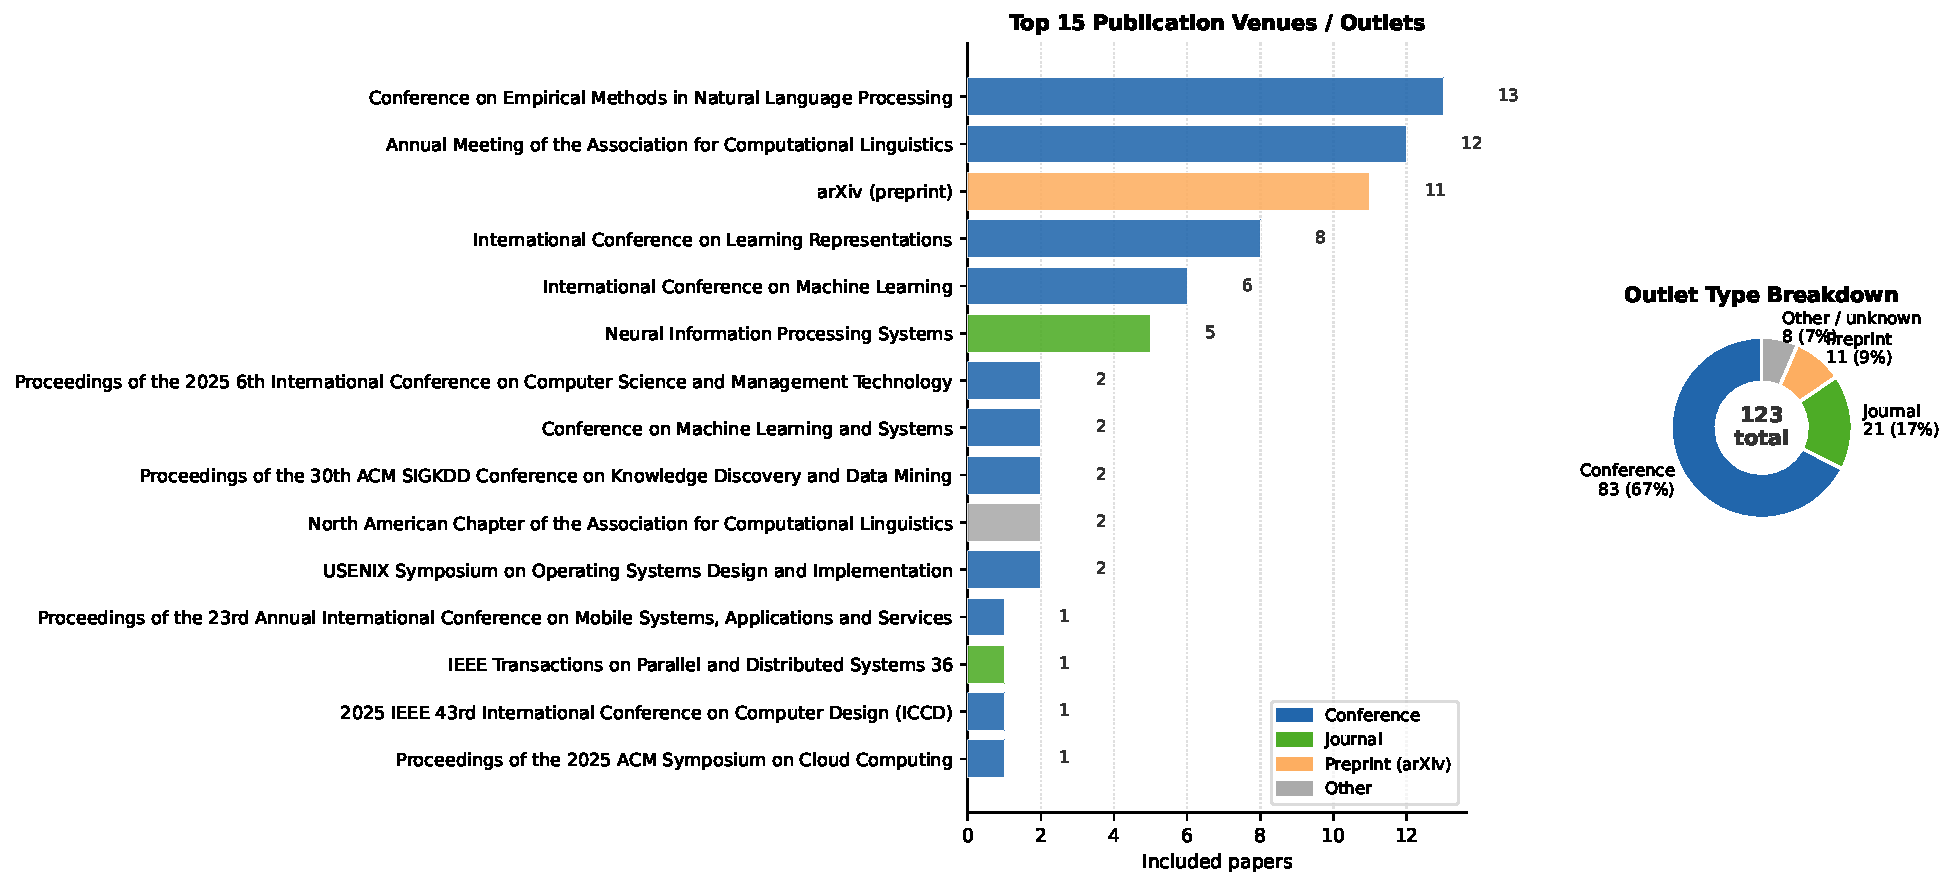
\includegraphics[width=1\linewidth]{figures/fig_slr5_venues.pdf}
  \caption{Venue distribution of the 464-paper enriched pool (an intermediate
           funnel stage prior to full-text review and quality appraisal;
           \emph{not} the final 123-paper corpus). ACL/EMNLP comprises the
           largest venue category (25 papers), followed by arXiv preprints
           (9), NeurIPS (8), and ICML/MLSys (7).}
  \label{fig:venues}
\end{figure}

\begin{figure}[H]
  \centering
  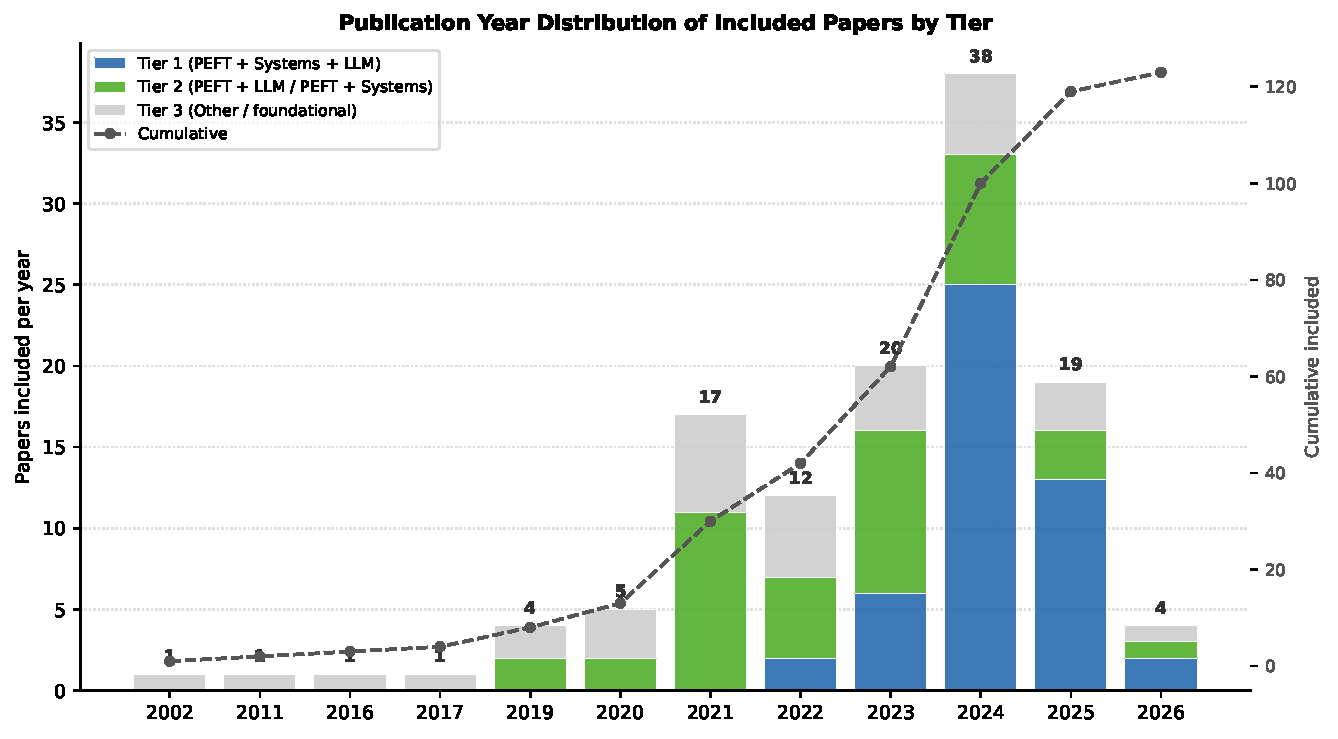
\includegraphics[width=1\linewidth]{figures/fig_slr3_year_distribution.pdf}
  \caption{Year distribution of the 123-paper reviewed corpus,
           showing the acceleration of publication volume from 2023 onward.}
  \label{fig:bibliometric}
\end{figure}

The most densely covered concept-matrix dimension is \textbf{adapter
exchange} (present in the majority of the 123 papers), while
\textbf{peer-to-peer topology} and \textbf{discovery mechanism} remain the
least covered dimensions, directly motivating the gaps identified in
Section~\ref{sec:synthesis_gap}.

\subsection*{A.7 Abstract-Level Review}

Following Keshav~\cite{Keshav2007}, the author conducted an abstract-level
review across all 552 records (464 enriched corpus records --- the 32
deprioritised low-citation arXiv preprints in the rescue file were confirmed
excluded and were not reinstated --- plus 88 records from forward citation
snowballing on Scopus and WoS that were title-screened and added to the
review). To support decision
consistency across a corpus of this size, each abstract was accompanied by an
automated advisory note providing a one-sentence summary, a relevance
assessment relative to the three core themes, and a preliminary KEEP / SKIP /
DEFER recommendation. These notes served as a consistency aid; all final
decisions were made by the author after independent assessment. The model
identifier, the automated suggestion, and the author's final decision are
logged per record in \texttt{S7b\_abstract\_reviewed\_final.csv} to support
reproducibility checks.

\begin{table}[H]
\centering
\caption{Abstract review outcomes, final consolidated classification (552
records reviewed). KEEP (214) and SKIP (338) sum to the 552 reviewed; the 173
intermediate second-pass DEFER records are subsumed within the 338 SKIP in
this final consolidation. These 173 borderline-DEFER records were, however,
also carried into the full-text review queue (214 KEEP ${}+{}$ 173 DEFER =
387 queued; see text), and a subset was read in full during full-text
review before being excluded at final curation — none reached the
data-extraction stage.}
\label{tab:abstract}
\begin{tabular}{lrr}
\toprule
\textbf{Decision} & \textbf{\textit{N}} & \textbf{\%} \\
\midrule
KEEP (included in the full-text review queue)  & 214 & 38.8 \\
SKIP (excluded, or full text not retrieved)    & 338 & 61.2 \\
\midrule
\textbf{Total reviewed}                        & \textbf{552} & \\
\bottomrule
\end{tabular}
\end{table}

KEEP papers were exported for full-text review via RIS format
(\texttt{08\_zotero\_ready\_2026-05-02.ris}, 214 entries). The full-text
review queue (\texttt{09\_fulltext\_review\_queue\_2026-05-02.csv}),
compiled from the 214 KEEP and the 173 borderline-DEFER records, contains
\textbf{387} records; of these, \textbf{190} proceeded to data extraction (all
KEEP-origin; no DEFER-origin records reached extraction) and \textbf{197} were
excluded (24 KEEP-origin, full text unavailable; 173 DEFER-origin, not taken
further). A
separate manual Scopus/WoS cross-validation top-up of \textbf{34} records
entered directly at the extraction stage, bypassing this full-text queue
(none were ultimately retained in the final 123), bringing the extraction
set to \textbf{224} (\texttt{11\_data\_extraction\_2026-05-12.csv}). A subset of the
queued DEFER records was read in full during this phase but was excluded at
the final curation step (Appendix~\ref{app:search_log}, Table~\ref{tab:search_log}).
Every record and its per-stage membership are traceable in the unified
pipeline file (\texttt{pipeline\_unified.csv}). The final reading list
(\texttt{13\_final\_reading\_list\_2026-05-12.csv}) is the authoritative
evidentiary base: \textbf{only the 123 papers it lists} entered the final
inclusion set for this review. Records from earlier pipeline stages whose full
text was not obtained (whether marked \texttt{DEFER} or left un-assessed, and
in each case because no PDF was downloaded) were not included in the final
reading list. The evidence presented in this review therefore rests solely on
these 123 papers.

% =============================================================================
%  Appendix B — Undermind Group Search Prompts
% =============================================================================

\section[\appendixname~\thesection]{Undermind Group Search Prompts}
\label{app:undermind}

The following six prompts were submitted verbatim to Undermind (undermind.ai) to
retrieve candidate papers for Groups G1--G6 of the pre-validated corpus described in
Section~\ref{sec:methodology:search}. Undermind was used exclusively for candidate
\textit{retrieval}; all inclusion and exclusion decisions were made by the author
through manual assessment of each returned record. The prompts are reproduced here
in their entirety for transparency and reproducibility.

% -----------------------------------------------------------------------
\subsection*{Group 1 — Advanced Adapter Architectures \& PEFT Methods}
\label{app:undermind:g1}

\begin{quote}\small
I am researching parameter-efficient fine-tuning (PEFT) methods for large language
models, building on the foundational work of Houlsby et al.\ (2019) on bottleneck
adapters and Hu et al.\ (2022) on LoRA (Low-Rank Adaptation). I am looking for
papers that extend, improve, or propose alternatives to these methods, including but
not limited to: QLoRA (quantized LoRA), DoRA, IA\textsuperscript{3}, prefix tuning,
prompt tuning, BitFit, sparse adapters, hypernetwork-based adapters (HyperFormer),
adapter pruning, rank-adaptive LoRA, VeRA, and methods that combine adapters with
quantization or knowledge distillation. I am specifically interested in works that
analyze the expressiveness, rank selection, or composability of low-rank and bottleneck
adapter modules in transformer architectures (encoder-only, decoder-only, and
encoder-decoder). Please retrieve the most cited and most recent SOTA papers in this
space, including survey papers beyond Han et al.\ (2024, TMLR).
\end{quote}

% -----------------------------------------------------------------------
\subsection*{Group 2 — Multi-Task Learning \& Adapter Composition}
\label{app:undermind:g2}

\begin{quote}\small
I am researching multi-task learning with adapter modules and task composition
techniques for transformer-based language models, building on AdapterFusion (Pfeiffer
et al., 2021, EACL) and AdapterHub (Pfeiffer et al., 2020, EMNLP). I want to find
papers on: non-destructive composition of multiple task-specific adapters, adapter
stacking and fusion strategies, hypernetwork-based multi-task adapter generation
(e.g., HyperFormer, HyperFormer++), multi-task adapter routing, knowledge transfer
between adapters, continual learning with adapters, task arithmetic and model merging
(e.g., TIES-merging, DARE), and zero-shot or few-shot generalization via adapter
composition. I am also interested in works comparing centralized multi-task
fine-tuning with modular adapter-based multi-task approaches. Please retrieve the
most relevant and highly cited SOTA papers, including recent 2023--2025 works.
\end{quote}

% -----------------------------------------------------------------------
\subsection*{Group 3 — P2P Networks \& Decentralised Systems for ML}
\label{app:undermind:g3}

\begin{quote}\small
I am researching peer-to-peer (P2P) and decentralized distributed systems applied to
machine learning and deep learning, building on: Petals (Borzunov et al., 2022/2023,
ACL/NeurIPS) for collaborative LLM inference, \v{S}ajina et al.\ (2024, Future
Generation Computer Systems) on multi-task P2P learning with encoder-only
transformers, and \v{S}ajina (2021, University of Rijeka doctoral thesis) on
peer-to-peer deep learning. I am looking for papers on: decentralized model training
and inference over P2P overlays, gossip-based and DHT-based protocols for model or
parameter sharing, capability-aware peer discovery in ML networks, decentralized
federated learning without a central server, split inference across heterogeneous edge
nodes, bandwidth-aware and latency-aware distributed inference, and decentralized
model marketplaces. Please also include foundational P2P systems papers (Chord,
Kademlia, BitTorrent) that are relevant to designing distributed ML systems. Retrieve
the most relevant SOTA papers from 2018--2025.
\end{quote}

% -----------------------------------------------------------------------
\subsection*{Group 4 — Efficient Inference \& Multi-Adapter Serving}
\label{app:undermind:g4}

\begin{quote}\small
I am researching efficient inference systems for large language models with a focus
on serving multiple adapters (LoRA or bottleneck) simultaneously over a single frozen
base model, building on S-LoRA (Sheng et al., 2024, MLSys) and Petals (Borzunov
et al., 2023). I want to find papers on: multi-tenant LLM serving with adapter
multiplexing, dynamic adapter loading and swapping at inference time, memory-efficient
batching strategies for adapter inference (e.g., unified paging, continuous batching),
KV cache management under adapter heterogeneity, model serving on constrained hardware
(edge devices, commodity GPUs), speculative decoding with adapters, pipeline
parallelism for adapter-augmented models, and systems like vLLM, Punica, AlpaServe,
FlexGen, and EdgeServe. I am also interested in work on adapter caching, prefetching
strategies, and latency-accuracy tradeoffs in multi-adapter inference. Please retrieve
the most relevant and most cited SOTA papers from 2020--2025, prioritizing MLSys,
OSDI, EuroSys, SOSP, and NSDI venues.
\end{quote}

% -----------------------------------------------------------------------
\subsection*{Group 5 — Routing \& Mixture-of-Experts}
\label{app:undermind:g5}

\begin{quote}\small
I am researching routing mechanisms and Mixture-of-Experts (MoE) architectures
applied to transformer models, with a focus on their connection to adapter-based and
modular multi-task learning. My starting point includes AdapterFusion (Pfeiffer et
al., 2021) and S-LoRA (Sheng et al., 2024). I want to find papers on: sparse MoE
routing in transformers (Switch Transformer, GShard, GLaM, Mixtral), expert choice
routing and load balancing strategies (Zhou et al., 2022), soft routing and
differentiable gating mechanisms, Mixture-of-Adapters (MoA) and MoE applied
specifically to PEFT/LoRA modules (e.g., MoLoRA, MixLoRA, Adapter-X by Li et al.\
2024), task-conditioned adapter routing, learned routing without task identity, and
routing in decentralized or federated settings. I am also interested in theoretical
analyses of routing stability, collapse, and capacity. Please retrieve the most
relevant SOTA papers from 2020--2025, including both NLP and systems-focused works.
\end{quote}

% -----------------------------------------------------------------------
\subsection*{Group 6 — Federated Learning \& Privacy-Preserving Adaptation}
\label{app:undermind:g6}

\begin{quote}\small
I am researching federated learning with a focus on privacy-preserving fine-tuning and
adapter-based personalization for transformer models. I am looking for papers that
connect to the proposed research on decentralized adapter systems. Starting from the general
federated learning literature (FedAvg by McMahan et al., 2017; FedProx by Li et al.,
2020), I want papers on: federated fine-tuning of large language models using LoRA or
adapter modules (e.g., FedPEFT, FedAdapter), personalized federated learning with
heterogeneous local models (pFedMMA, per-FedAvg), non-IID data distributions and
their effect on adapter convergence, differential privacy in federated adapter
training, cross-silo vs.\ cross-device federated learning for NLP, medical and
clinical federated learning benchmarks (FLamby, MIMIC), communication-efficient
federated learning with sparse or compressed updates, and split learning with adapter
modules. Please retrieve the most relevant and most cited SOTA papers from 2017--2025,
prioritizing works that explicitly address heterogeneous data or privacy constraints in
adapter or PEFT contexts.
\end{quote}

% =============================================================================
%  Appendix B — Manual Database Search Queries
% =============================================================================

\section[\appendixname~\thesection]{Manual Database Search Queries}
\label{app:db_queries}

Scopus (Elsevier) and Web of Science (Clarivate) were queried manually as part of the
snowballing and enrichment stages described in Appendix~\ref{sec:appendix:corpus_pipeline}.
Ten advanced search queries were executed on each platform. In Scopus, results were
filtered to journal articles and conference proceedings (\texttt{SRCTYPE("j" OR "p")}).
In WoS, Topic-field (\texttt{TS=}) queries were used with equivalent year filters.
The WoS Starter API was subsequently used in a \textit{post-hoc enrichment role} only
--- to append WoS accession numbers and citation counts to already-retrieved records ---
and was not a source of new candidates. All raw result sets from both platforms are
archived alongside the \texttt{slr\_engine} repository (\texttt{exports/scopus/} and
\texttt{exports/wos/}); access is detailed in the Data Availability statement.

% -----------------------------------------------------------------------
\subsection*{Scopus Advanced Search Queries}
\label{app:db_queries:scopus}

\paragraph{Q1 — Core Adapter-Based NLP.}
\begin{verbatim}
TITLE-ABS-KEY(("adapter" OR "adapters" OR "LoRA" OR "low-rank")
AND ("parameter-efficient" OR "PEFT" OR "parameter efficient")
AND ("NLP" OR "natural language processing" OR "transformer"))
AND SRCTYPE("j" OR "p")
AND PUBYEAR > 2018
\end{verbatim}

\paragraph{Q2 — Multi-Task Learning with Transformers.}
\begin{verbatim}
TITLE-ABS-KEY((("adapter*" OR "LoRA" OR "parameter-efficient fine-tuning")
AND ("multi-task" OR "multitask" OR "multi-adapter")
AND ("inference" OR "serving" OR "deployment" OR "edge")))
AND SRCTYPE(j OR p)
AND PUBYEAR > 2020
AND NOT TITLE-ABS-KEY(("medical" OR "healthcare" OR "clinical"
    OR "sentiment" OR "recommendation"))
\end{verbatim}

\paragraph{Q3 — Peer-to-Peer \& Distributed NLP.}
\begin{verbatim}
TITLE-ABS-KEY(("peer-to-peer" OR "P2P" OR "decentralized" OR "federated")
AND ("learning" OR "training" OR "inference")
AND ("NLP" OR "natural language" OR "machine learning" OR "deep learning"))
AND SRCTYPE("j" OR "p")
AND PUBYEAR > 2017
\end{verbatim}

\paragraph{Q4 — Adapter Fusion \& Dynamic Routing.}
\begin{verbatim}
TITLE-ABS-KEY(("adapter" OR "adapters")
AND ("fusion" OR "routing" OR "dynamic" OR "mixture-of-experts"
    OR "MoE" OR "gating"))
AND SRCTYPE("j" OR "p")
AND PUBYEAR > 2020
\end{verbatim}

\paragraph{Q5 — Parameter-Efficient Multi-Task Transformers.}
\begin{verbatim}
TITLE-ABS-KEY(("parameter-efficient" OR "PEFT" OR "efficient adaptation")
AND ("multi-task" OR "multitask")
AND ("transformer" OR "pre-trained models"))
AND SRCTYPE("j" OR "p")
AND PUBYEAR > 2019
\end{verbatim}

\paragraph{Q6 — Modular Inference \& Task Switching.}
\begin{verbatim}
TITLE-ABS-KEY(("modular" OR "modularity")
AND ("inference" OR "inference time")
AND ("adapter" OR "task-specific" OR "lightweight modules"))
AND SRCTYPE("j" OR "p")
AND PUBYEAR > 2018
\end{verbatim}

\paragraph{Q7 — Agent-Based Collaborative Learning.}
\begin{verbatim}
TITLE-ABS-KEY(("agent" OR "agents" OR "node" OR "nodes")
AND ("collaborative" OR "collaboration" OR "decentralized")
AND ("deep learning" OR "neural network" OR "model training"))
AND SRCTYPE("j" OR "p")
AND PUBYEAR > 2017
\end{verbatim}

\paragraph{Q8 — NL-to-SQL with Adapters.}
\begin{verbatim}
TITLE-ABS-KEY(("NL-to-SQL" OR "semantic parsing"
    OR "natural language to SQL")
AND ("adapter" OR "fine-tun*" OR "parameter-efficient" OR "efficient"))
AND SRCTYPE("j" OR "p")
AND PUBYEAR > 2019
\end{verbatim}

\paragraph{Q9 — Sequence Labelling \& Token Classification with PEFT.}
\begin{verbatim}
TITLE-ABS-KEY(("token classification" OR "NER"
    OR "named entity recognition" OR "sequence labeling")
AND ("adapter" OR "LoRA" OR "parameter-efficient" OR "PEFT"))
AND SRCTYPE("j" OR "p")
AND PUBYEAR > 2019
\end{verbatim}

\paragraph{Q10 — Frozen Base Model Paradigm.}
\begin{verbatim}
TITLE-ABS-KEY(("frozen" OR "freeze" OR "frozen base")
AND ("adapter" OR "efficient" OR "modular")
AND ("transfer learning" OR "fine-tun*"))
AND SRCTYPE("j" OR "p")
AND PUBYEAR > 2018
\end{verbatim}

% -----------------------------------------------------------------------
\subsection*{Web of Science Advanced Search Queries}
\label{app:db_queries:wos}

\paragraph{Q1 — Core Adapter-Based NLP.}
\begin{verbatim}
TS=(("adapter" OR "adapters" OR "LoRA" OR "low-rank")
AND ("parameter-efficient" OR "PEFT" OR "parameter efficient")
AND ("NLP" OR "natural language processing" OR "transformer"))
AND PY >= 2018
\end{verbatim}

\paragraph{Q2 — Multi-Task Adapter Inference.}
\begin{verbatim}
TS=((("adapter*" OR "LoRA" OR "PEFT")
AND ("multi-task" OR "multitask")
AND ("inference" OR "serving" OR "edge" OR "distributed")))
AND PY >= 2021
AND NOT TS=(("medical" OR "healthcare" OR "sentiment"))
\end{verbatim}

\paragraph{Q3 — Peer-to-Peer Distributed Learning.}
\begin{verbatim}
TS=(("peer-to-peer" OR "P2P" OR "decentralized" OR "federated")
AND ("learning" OR "training" OR "inference")
AND ("NLP" OR "natural language" OR "machine learning"
    OR "neural network"))
AND PY >= 2017
\end{verbatim}

\paragraph{Q4 — Adapter Fusion \& Routing Mechanisms.}
\begin{verbatim}
TS=(("adapter" OR "adapters")
AND ("fusion" OR "dynamic routing" OR "mixture-of-experts"
    OR "MoE" OR "gating"))
AND PY >= 2020
\end{verbatim}

\paragraph{Q5 — Modular Deep Learning.}
\begin{verbatim}
TS=(("modular" OR "modularity")
AND ("neural" OR "transformer" OR "deep learning")
AND ("inference" OR "task-specific" OR "lightweight"))
AND PY >= 2018
\end{verbatim}

\paragraph{Q6 — Agent-Based Collaborative ML.}
\begin{verbatim}
TS=(("agent" OR "agents" OR "distributed node*")
AND ("collaborative" OR "collaboration" OR "decentralized"
    OR "gossip")
AND ("deep learning" OR "machine learning"))
AND PY >= 2017
\end{verbatim}

\paragraph{Q7 — Memory-Efficient Multi-Task NLP.}
\begin{verbatim}
TS=(("multi-task" OR "multitask")
AND ("memory-efficient" OR "memory efficient"
    OR "parameter-efficient" OR "computational efficient")
AND ("NLP" OR "natural language" OR "transformer"))
AND PY >= 2018
\end{verbatim}

\paragraph{Q8 — Transfer Learning with Task Adaptation.}
\begin{verbatim}
TS=(("transfer learning" OR "fine-tun*")
AND ("adapter" OR "parameter-efficient" OR "LoRA")
AND ("NLP" OR "text" OR "language"))
AND PY >= 2019
\end{verbatim}

\paragraph{Q9 — Sequence Task Learning.}
\begin{verbatim}
TS=(("token classification" OR "NER" OR "named entity"
    OR "sequence labeling")
AND ("adapter" OR "fine-tun*" OR "efficient" OR "modular"))
AND PY >= 2019
\end{verbatim}

\paragraph{Q10 — Distributed Inference.}
\begin{verbatim}
TS=(("distributed" OR "decentralized")
AND ("inference" OR "inference time")
AND ("efficient" OR "modular" OR "lightweight"))
AND PY >= 2018
\end{verbatim}

% =============================================================================
%  Appendix C — Search Execution Log
% =============================================================================

\section[\appendixname~\thesection]{Search Execution Log}
\label{app:search_log}

This appendix provides a chronological account of every search activity performed
during corpus construction, together with record counts at each stage
(Table~\ref{tab:search_log}). The purpose
is to allow full reproduction or audit of the PRISMA flow by the reader or supervisor.
The audited final deliverables referenced below are committed to the
\texttt{slr\_engine} repository under
\texttt{snowballing/snowball\_output/}
(\url{https://github.com/vanjaluk8/slr_engine/tree/main/slr_engine/snowballing/snowball_output});
see the Data Availability statement for further repository access.

% -----------------------------------------------------------------------
\subsection*{D.1 — Search Timeline}
\label{app:search_log:timeline}


\begin{table}[H]
\centering
\small
\caption{Chronological search log with input and output record counts.}
\label{tab:search_log}
\begin{tabularx}{\textwidth}{@{}
  l
  X
  >{\raggedright}p{2.2cm}
  >{\raggedright\arraybackslash}p{3.8cm}
@{}}
\toprule
\textbf{Date} & \textbf{Activity} & \textbf{In} & \textbf{Out} \\
\midrule
2026-04-21 & Semantic Scholar API snowball on G0 seeds (backward + forward) &
  7 seeds & 1\,150 raw \\
2026-04-21 & Within-snowball deduplication (DOI + SS paper ID) &
  1\,150 & 972 \\
2026-04-21 & Title screening (Layer~1: year; Layer~2: keyword; Layer~3: LLM triage) &
  972 & 162 INCL, 791 EXCL, 19 UNCERT \\
2026-04-21 & Merge snowball INCLUDE with 352-paper pre-validated corpus (G0--G6);
  cross-deduplication & 514 & 502 \\
$\approx$2026-04-22 & Semantic Scholar / OpenAlex enrichment + topical-relevance filter &
  502 & 464 kept; 32 depri.; 6 excl. \\
$\approx$2026-04-28 & Abstract-level review, pass 1 (on the 464 corpus; AI-assisted,
  human decision) & 464 & 202 KEEP, 169 DEFER, 93 SKIP \\
2026-04-28/05-02 & Abstract review passes completed across the extended pool
  (464 $+$ 88 forward snowball records) & 552 & 214 KEEP, 173 DEFER, 165 SKIP \\
2026-05-02  & Fulltext review queue compiled from KEEP and borderline-DEFER records &
  KEEP/DEFER subset & 387 queued \\
2026-05-02  & Preliminary data extraction & 387 & 190 extracted \\
2026-05-08  & Forward citation snowball: Scopus (citing G0) &
  106 raw & 74 title-screened in \\
2026-05-08  & Forward citation snowball: Web of Science (citing G0) &
  20 raw  & 14 title-screened in \\
2026-05-08  & Forward snowball records added to abstract review (G\_SNOW\_F group) &
  88 added & 12 KEEP; 4 DEFER; 72 SKIP \\
2026-05-11  & DOI-based venue validation: Scopus (\texttt{M3\_scopus\_venue}) &
  172 DOIs & 172 matched \\
2026-05-11  & DOI-based venue validation: Web of Science (\texttt{M4\_wos\_venue}) &
  125 DOIs & 125 matched \\
2026-05-12  & Data-extraction top-up with manual Scopus/WoS additions &
  190 & 224 extracted (34 top-up) \\
2026-05-12  & Full-text reading, quality assessment, and final curation (final
  reading list is the authoritative evidence base) &
  --- & 123 final \\
\bottomrule
\end{tabularx}
\end{table}

% -----------------------------------------------------------------------
\subsection*{D.2 — Automated Citation Snowballing}
\label{app:search_log:snowball}

Citation snowballing was executed programmatically on \textbf{2026-04-21} via the
Semantic Scholar Academic Graph API, supplemented by Scopus and ACL Anthology engines,
following the procedure of Wohlin et al.~\cite{Wohlin2014}. The G0 corpus comprises nine seed
papers; seven of these were submitted for both backward (reference list) and forward (citing
papers) retrieval via the Semantic Scholar API. The remaining two seeds were
excluded from this automated pass for documented reasons: the doctoral thesis
of \v{S}ajina~\cite{Sajina2025} (University of Rijeka repository object
infri:1394) is documented in the institutional repository rather than an
API-indexed DOI, so its record was incorporated through the pre-validated
G0--G6 corpus rather than automated retrieval; \v{S}ajina et
al.~\cite{Sajina2024} was evaluated but excluded because its forward citations
yielded no new usable candidates and its backward citations substantially
overlapped with papers already retrieved through the other seven seeds. Raw API
responses yielded \textbf{1,150 candidate records}; after deduplication by DOI and
Semantic Scholar paper identifier, \textbf{972 unique records} entered title screening.
Screening decisions are logged in \texttt{log\_screening\_2026-04-21.json}; per-seed
retrieval counts are in \texttt{log\_retrieval\_2026-04-21.json}.

% -----------------------------------------------------------------------
\subsection*{D.3 — Forward Citation Snowballing (Scopus and WoS)}
\label{app:search_log:forward}

On \textbf{2026-05-08}, a supplementary forward snowball was conducted by manually
querying the Scopus and Web of Science interfaces for papers citing any of the G0 seed
papers. This step retrieved \textbf{106 records from Scopus}
(\texttt{MANUAL\_FORWARD\_SCOPUS\_0805.csv}) and \textbf{20 records from WoS}
(\texttt{M1\_forward\_wos\_2026-05-08.txt}). After manual title screening, \textbf{88
records} (74 Scopus + 14 WoS) passed the relevance threshold and were appended to the
abstract review pool under the source group \texttt{G\_SNOW\_F}. These 88 records
bypassed the automated enrichment filter and entered the review directly. Of the 88,
\textbf{12 were assigned KEEP}, 4 were assigned DEFER, and 72 were SKIP at abstract
review; the 4 DEFER records were resolved to SKIP in the final consolidation.
None of the 88 \texttt{G\_SNOW\_F} records survived to the final 123-record list:
although the 12 KEEP records entered the full-text queue (8 reaching data
extraction), all were excluded at the eligibility stage, so the forward branch
contributes \textbf{0} records to the final list.

% -----------------------------------------------------------------------
\subsection*{D.4 — Manual Database Cross-Validation}
\label{app:search_log:crossval}

To verify completeness, the ten WoS and ten Scopus advanced queries documented in
Appendix~C were also executed manually against the live database interfaces.
\textbf{Scopus} returned \textbf{172 records}
(\texttt{11\_MANUAL\_SCOPUS\_export\_1105.csv}); \textbf{Web of Science} returned
\textbf{125 records} (\texttt{11\_MANUAL\_WOS\_export\_1105.txt}).

Cross-referencing the 125 WoS records against the existing merged corpus revealed that
all candidates were already present via the Semantic Scholar and Scopus retrieval
pipeline; \textbf{zero new candidates} were identified from the WoS manual search.
This outcome is consistent with the known indexing overlap between WoS and Scopus for
the PEFT, NLP systems, and distributed ML literature: Scopus coverage is broader for
conference proceedings from ACL, NeurIPS, ICML, and MLSys venues, which dominate this
review's citation landscape. The WoS manual search therefore served as a \textit{coverage
cross-check} rather than a source of new records, confirming that the Scopus-dominated
retrieval pipeline achieved comprehensive coverage of the target literature.

% -----------------------------------------------------------------------
\subsection*{D.5 — DOI-Based Venue Verification}
\label{app:search_log:doi}

Following full-text reading, the DOIs of candidate papers were submitted in batch to
Scopus and WoS to retrieve authoritative venue, publication year, and citation-count
metadata. The Scopus batch returned \textbf{172 records}
(\texttt{M3\_scopus\_venue\_validation\_2026-05-11.csv}); the WoS batch returned
\textbf{125 records} (\texttt{M4\_wos\_venue\_validation\_2026-05-11.txt}). These
files served exclusively as metadata enrichment sources: they appended WoS accession
numbers and confirmed Scopus EIDs to records already in the reading pool, and were not
used to introduce new candidates.

% -----------------------------------------------------------------------
\subsection*{D.6 — Manual PDF and Venue Check}
\label{app:search_log:pdf}

A subset of candidate papers had been initially downloaded from the arXiv preprint
server. As a final quality step, each arXiv download was manually checked against
Google Scholar, Semantic Scholar, and the ACL Anthology to determine whether a
peer-reviewed published version existed. Where a published venue was identified and
the PDF was publicly accessible, the preprint was replaced with the official published
version and the venue metadata was updated accordingly. After this step,
\textbf{18 papers} in the final 123-paper reading list retained an arXiv source
(\texttt{source = ARXIV} in \texttt{13\_final\_reading\_list\_2026-05-12.csv}),
either because no published version was found or because the accepted manuscript was
not separately accessible. (This ``18'' figure reports the \emph{retrieval source};
a separate, narrower count of \textbf{11 records} cited in
Section~\ref{sec:conclusion:threats} reports \emph{venue status}---records
whose current indexed venue remains arXiv and for which no peer-reviewed
published version was identified at any retrieval stage.) A further \textbf{4 records} have no source annotation,
reflecting papers added from curated references whose primary retrieval provenance was
not logged in the pipeline output files.
